\section{Evaluation}
\label{sec:evaluation}

The evaluation examines whether \system can advance agentic skill analysis
from security screening to evidence based security adjudication. All results
use the fixed 776-case ProvBench corpus and the frozen configuration described
in Section~\ref{sec:benchmark-setup}. The evaluation measures overall security
decisions and evidence recovery, isolates the contribution of the main
analysis components, examines the remaining evidence and execution
boundaries, and compares \system with existing skill security analyzers.


\subsection{Overall Effectiveness}
\label{sec:eval-overall}

\textbf{Security decisions.}
The full \system configuration identifies 291 of the 398 confirmed violations
and correctly classifies 339 of the 378 remaining cases. Precision is 0.882,
recall is 0.731, and F1 is 0.799. All 39 false positives occur on trusted
allowed cases. None of the 179 benign lookalikes is classified as a violation.

Static instruction analysis favors recall over precision. Static
screening identifies all 398 confirmed violations and reaches 0.917 F1, while
72 nonviolations are escalated. Full \system reduces the false positive count
from 72 to 39 and removes all false positives on benign lookalikes. Runtime
provenance, alignment, evidence closure, and policy evaluation impose a
stricter requirement for the final security decision.




\textbf{Evidence recovery.}
Table~\ref{tab:evidence-recovery} reports the evidence recovered by the full
configuration. Violation closure reaches 0.863 precision, 0.618 recall, and
0.720 F1. Evidence closure reaches 1.000 precision, 0.616 recall, and 0.762
F1. Evidence closure succeeds for 245 of the 398 confirmed violations.

\begin{table}[t]
\caption{Evidence recovery of full \system on ProvBench.}
\label{tab:evidence-recovery}
\centering
\small
\setlength{\tabcolsep}{5pt}
\renewcommand{\arraystretch}{1.12}
\begin{tabular*}{\columnwidth}{@{\extracolsep{\fill}}lccc}
\toprule
\textbf{Metric}
& \textbf{Precision}
& \textbf{Recall}
& \textbf{F1} \\
\midrule
Violation closure
& 0.863 & 0.618 & 0.720 \\

Evidence closure
& 1.000 & 0.616 & 0.762 \\
\addlinespace[2pt]

Source object
& 0.500 & 0.506 & 0.503 \\

Sink object
& 0.718 & 0.367 & 0.486 \\

Edge operation
& 0.892 & 0.426 & 0.577 \\

Minimal witness
& 0.222 & 0.436 & 0.294 \\
\bottomrule
\end{tabular*}
\end{table}

Evidence closure precision is 1.000 and recall is 0.616. The closure contract
requires a protected source, admissible carrier relations, an applicable
terminal operation, and sufficient terminal evidence before reporting a
closed path.

Provenance fidelity applies a stricter requirement to the recovered
explanation. Source object F1 is 0.503, sink object F1 is 0.486, edge
operation F1 is 0.577, and minimal witness F1 is 0.294.
Section~\ref{sec:eval-boundaries} examines the remaining structural gap.


\textbf{Analysis cost.}
Cost measurements use the same frozen run as the reported security and
evidence results. Median latency is 80.7 seconds per case, and the 95th
percentile is 391.2 seconds. A median case uses 9 LLM requests and 24,546
tokens. The 95th percentile reaches 14 requests and 53,644 tokens. The median
runtime provenance graph contains 259 nodes and 287 edges.

The measured latency makes the full system better suited to offline security
analysis than to real-time screening. Applications with stricter latency
requirements can use the static stage for initial screening.


\subsection{Component Contributions}
\label{sec:eval-ablation}

Figure~\ref{fig:ablation} isolates the contribution of static instruction
analysis, runtime evidence, cross layer alignment, and policy evaluation. All
variants operate on the same 776 ProvBench cases.

\begin{figure}[H]
    \centering
    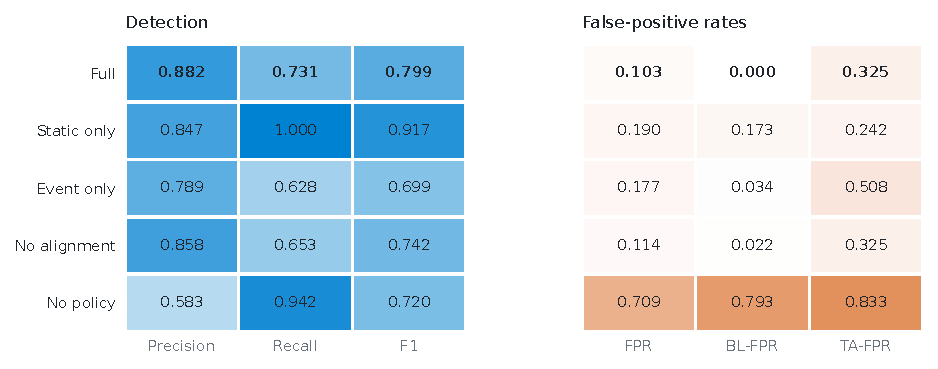
\includegraphics[width=\columnwidth]{figures/fig5_ablation.pdf}
    \caption{Ablation of \system components on ProvBench.}
    \label{fig:ablation}
\end{figure}

\textbf{Static instruction screening.}
Static only analysis reaches 0.847 precision, 1.000 recall, and 0.917 F1.
Static instruction analysis identifies every confirmed violation and provides
the high recall screening stage of \system. Static screening also produces an
overall false positive rate of 0.190 and a benign lookalike false positive
rate of 0.173.

Full adjudication lowers the overall false positive rate to 0.103 and the
benign lookalike false positive rate to zero. Static instruction analysis
identifies security relevant capabilities. Full adjudication requires runtime
and policy evidence before assigning a violation.


\textbf{Runtime evidence.}
Event only analysis reaches 0.789 precision, 0.628 recall, and 0.699 F1.
The trusted allowed false positive rate reaches 0.508. Runtime events establish
file access, process execution, data movement, and external communication.
Instruction provenance supplies the referenced entities, operation,
conditions, and modality needed to interpret the observed behavior. Static and runtime evidence serve different roles. Runtime provenance records behavior exercised
during bounded execution and tracks protected sources through observed
carriers.


\textbf{Cross layer alignment.}
Removing alignment reduces F1 from 0.799 to 0.742. Precision becomes 0.858
and recall becomes 0.653. Cross layer alignment associates instruction
entities and operations with compatible runtime evidence before closure is
evaluated. Aligned provenance distinguishes behavior expressed by the skill from behavior
observed during execution. Closure operates on relations supported across the two provenance views.


\textbf{Policy evaluation.}
The No policy variant retains instruction and runtime evidence while removing
policy adjudication. Precision falls to 0.583, recall rises to 0.942, and F1
becomes 0.720. The overall false positive rate reaches 0.709. Benign lookalike
and trusted allowed false positive rates reach 0.793 and 0.833. The policy ablation separates observed flow from policy violation. Authorized
authentication, approved delivery, trusted service interaction, and permitted
state modification can contain genuine source-to-sink flows. Provenance
establishes the supported flow. Policy evaluation assigns the security meaning
of the supported flow.


\subsection{Evidence Quality and Error Analysis}
\label{sec:eval-boundaries}

The recovered evidence supports security decisions at the level most relevant
to analyst review. For each path, \system records the protected source,
observed carriers, terminal operation, destination, supporting instruction
evidence, policy state, and execution coverage. We next examine the
granularity of these explanations and the cases in which a final violation is
not established.


\textbf{Evidence granularity.}
\system captures the security relevant portion of a runtime path: where
protected data originates, how it is carried during execution, which terminal
operation acts on it, and where that operation is directed. Intermediate state
can remain at the carrier level when exact object identity is unavailable.

Consider a credential transfer that reads a synthetic secret, stages the
value, constructs an outbound payload, and sends the payload to a controlled
receiver. \system recovers the protected source, outbound carrier, send
operation, destination, and supporting instruction evidence. The resulting
witness directly explains why the observed transfer constitutes a
confidentiality violation.


\textbf{Policy distinction.}
Full \system produces no false positives on the 179 benign lookalikes. Its 39
false positives all occur on trusted allowed cases, where security relevant
operations are present but permitted by the scenario. The remaining precision
challenge is therefore concentrated in authorization rather than in
distinguishing benign lookalikes from prohibited flows.

The policy ablation makes this distinction visible. Removing policy evaluation
raises the false positive rate on trusted allowed cases from 0.325 to 0.833.
Policy information is thus important when permitted and prohibited workflows
contain similar sources, operations, and destinations.


\textbf{Unresolved violations.}
The 107 false negatives provide a clear view of where additional runtime
evidence is needed. Among them, 103 recover the expected protected source.
The missing evidence is concentrated at the terminal end of the path.

In 100 of these 103 cases, the protected value is observed in the LLM context.
The remaining 3 cases also expose the value through an HTTP body. In all 103
cases, source evidence is present, while the expected terminal operation is
not observed during bounded execution.

The dominant false negative is  a partially realized runtime path: \system
observes the protected source and its movement through runtime carriers, while
the execution stops short of the local state change or external operation
needed to establish the complete violation.

\begin{table}[t]
\caption{Expected terminals in 103 unresolved violations.}
\label{tab:fn-realization}
\centering
\small
\setlength{\tabcolsep}{5pt}
\renewcommand{\arraystretch}{1.12}
\begin{tabular*}{\columnwidth}{@{\extracolsep{\fill}}lr}
\toprule
\textbf{Expected terminal family}
& \textbf{Cases} \\
\midrule
Destructive local state
& 24 \\

Permission state
& 23 \\

Instruction state
& 21 \\

Persistence state
& 20 \\

Other nonlocal terminal
& 15 \\
\midrule
Total
& 103 \\
\bottomrule
\end{tabular*}
\end{table}

Table~\ref{tab:fn-realization} shows that 88 of the 103 cases involve local
state operations: destructive overwrites, permission updates, instruction
state changes, or persistence updates. The protected source is already visible
in the runtime evidence before these expected terminal operations.

The other 15 cases involve nonlocal operations such as requests, archives,
helper commands, and jobs. Their protected sources are also observed, while
the expected terminal action is not present in the recovered execution.

The remaining 4 false negatives arise outside this dominant pattern. Two reach
the expected target without an observable tainted carrier, one reaches the
execution budget before the decisive sink, and one depends on an unavailable
environment or dependency.


\textbf{Carrier coverage.}
Confirmed chain recall reaches 0.567 for plain text requests, 0.526 for
filtered CSV carriers, 0.518 for model prompt and response carriers, and 0.532
for package archives. These results show that \system can recover
source-to-sink evidence across several distinct data carrying surfaces rather
than relying on a single transport representation.

Local state transitions such as overwrite, permission, startup, and
instruction state updates account for most of the remaining coverage gap.
Improving observation of these state changes would extend the same provenance
analysis to a broader class of integrity and persistence behaviors.



\subsection{Comparison with Skill Analysis Tools}
\label{sec:eval-baselines}

\textbf{Baseline setup.}
The external baseline implementations were frozen from their August 9, 2026
repository snapshots. Each baseline was evaluated through its native skill
analysis workflow without changing the baseline detection logic.

AI-Infra-Guard is evaluated through its official Skill-Scan workflow.
AI-Infra-Guard performs LLM assisted code and instruction auditing over agent
skill packages and exports structured security findings.

Cisco Skill Scanner is evaluated with LLM analysis enabled. The Cisco scanner
combines deterministic security patterns, semantic model analysis, and
dataflow oriented checks for broad skill threat screening.

SkillScan is evaluated through its complete native scan workflow. SkillScan
first performs static security auditing, then runs LLM behavioral prediction,
and finally executes the sandbox test stage in Docker. The formal evaluation
environment provides both the configured model endpoint and Docker runtime, so
all three SkillScan stages participate in the reported baseline result.

The three baselines cover complementary approaches to existing skill
security analysis. AI-Infra-Guard emphasizes LLM assisted security auditing,
Cisco combines rule, semantic, and dataflow analysis, and SkillScan combines
static auditing, behavioral prediction, and sandbox execution. The comparison
uses the sample level binary security decision exported by each complete
configuration.

\begin{table}[H]
\caption{Binary security decisions on ProvBench.}
\label{tab:baseline-comparison}
\centering
\scriptsize
\setlength{\tabcolsep}{3.2pt}
\renewcommand{\arraystretch}{1.12}
\begin{threeparttable}
\begin{tabular*}{\columnwidth}{@{\extracolsep{\fill}}lccccc}
\toprule
\textbf{System}
& \textbf{TP/TN}
& \textbf{FP/FN}
& \textbf{P}
& \textbf{R}
& \textbf{F1} \\
\midrule

AI-Infra-Guard
& 101/373
& 5/297
& 0.953
& 0.254
& 0.401 \\

Cisco Skill Scanner
& 312/340
& 38/86
& 0.891
& 0.784
& 0.834 \\

SkillScan
& 144/360
& 18/254
& 0.889
& 0.362
& 0.514 \\

\midrule

\system\ Static
& 398/306
& 72/0
& 0.847
& 1.000
& \textbf{0.917} \\

\system\ Full
& 291/339
& 39/107
& 0.882
& 0.731
& 0.799 \\

\bottomrule
\end{tabular*}

\begin{tablenotes}[flushleft]
\scriptsize
\item \textit{Note:}
TP/TN denotes true positives and true negatives;
FP/FN denotes false positives and false negatives;
P and R denote precision and recall.
\end{tablenotes}
\end{threeparttable}
\end{table}



The external baselines exhibit different screening tradeoffs. Cisco Skill
Scanner reaches the strongest external F1 at 0.834. AI-Infra-Guard favors
precision, reaching 0.953 precision with 0.254 recall, while SkillScan reaches
0.514 F1.

The static stage of \system provides the strongest binary screening result in
Table~\ref{tab:baseline-comparison}, with 1.000 recall and 0.917 F1. Screening
performance is not the limiting factor in \system. The full
configuration begins from this high recall candidate set and applies runtime
provenance, cross layer alignment, evidence closure, and policy evaluation
before confirming a violation.

The additional evidence requirements change the operating point from screening
to adjudication. Relative to static screening, full \system reduces false
positives from 72 to 39, raises precision from 0.847 to 0.882, and reduces the
benign lookalike false positive rate from 0.173 to zero. The resulting binary
F1 is 0.799 because 107 confirmed violations lack sufficient runtime evidence
for final closure under bounded execution.

Binary F1 captures only one part of the comparison. The external
baselines terminate at a security finding or sample level decision. Full
\system additionally determines whether the decision is supported by a
protected source, an observed carrier path, a terminal operation, policy
context, and an explicit coverage state. On ProvBench, \system recovers
evidence supported source-to-sink closures for 61.6\% of confirmed violations
and produces no false closures on the 179 benign lookalikes.